\documentclass{article}

% if you need to pass options to natbib, use, e.g.:
     \PassOptionsToPackage{numbers, sort&compress}{natbib}
% before loading neurips_2021

% ready for submission
\usepackage{neurips_2021}

% to compile a preprint version, e.g., for submission to arXiv, add add the
% [preprint] option:
%     \usepackage[preprint]{neurips_2021}

% to compile a camera-ready version, add the [final] option, e.g.:
%     \usepackage[final]{neurips_2021}

% to avoid loading the natbib package, add option nonatbib:
%    \usepackage[nonatbib]{neurips_2021}

\usepackage[utf8]{inputenc} % allow utf-8 input
\usepackage[T1]{fontenc}    % use 8-bit T1 fonts
\usepackage{hyperref}       % hyperlinks
\usepackage{url}            % simple URL typesetting
\usepackage{booktabs}       % professional-quality tables
\usepackage{amsfonts}       % blackboard math symbols
\usepackage{nicefrac}       % compact symbols for 1/2, etc.
\usepackage{microtype}      % microtypography
\usepackage{xcolor}         % colors
%\usepackage{natbib}
\usepackage{graphicx}
\usepackage{soul}
\usepackage{enumitem}
\newcommand{\jd}[1]{\textcolor{orange}{[DJ: #1]}}
\newcommand{\jdtext}[1]{\textcolor{red}{#1}}
\newcommand{\aq}[1]{\textcolor{purple}{[AQ: #1]}}
\newcommand{\drop}[1]{\begin{scriptsize}{\textcolor{green}{[#1]}}\end{scriptsize}}


%Includes "References" in the table of contents
\usepackage[nottoc]{tocbibind}

%Import the natbib package and sets a bibliography style
%\usepackage[round,numbers]{natbib}
%\bibliographystyle{ksfh_nat}
\bibliographystyle{plainnat}

\title{Object Representations Guided By Optical Flow}

% The \author macro works with any number of authors. There are two commands
% used to separate the names and addresses of multiple authors: \And and \AND.
%
% Using \And between authors leaves it to LaTeX to determine where to break the
% lines. Using \AND forces a line break at that point. So, if LaTeX puts 3 of 4
% authors names on the first line, and the last on the second line, try using
% \AND instead of \And before the third author name.

\author{%
  David S.~Hippocampus\thanks{Use footnote for providing further information
    about author (webpage, alternative address)---\emph{not} for acknowledging
    funding agencies.} \\
  Department of Computer Science\\
  Cranberry-Lemon University\\
  Pittsburgh, PA 15213 \\
  \texttt{hippo@cs.cranberry-lemon.edu} \\
  % examples of more authors
  % \And
  % Coauthor \\
  % Affiliation \\
  % Address \\
  % \texttt{email} \\
  % \AND
  % Coauthor \\
  % Affiliation \\
  % Address \\
  % \texttt{email} \\
  % \And
  % Coauthor \\
  % Affiliation \\
  % Address \\
  % \texttt{email} \\
  % \And
  % Coauthor \\
  % Affiliation \\
  % Address \\
  % \texttt{email} \\
}

\begin{document}

\maketitle

  % and use this signal through optical flow approaches to learn object-centric representations. 
  
  % and optical flow approaches extract such signals very effectively.
  
  %This often involves training structured object encoders through reconstruction or prediction objectives or contrastive losses.  
  %Learning object-centric representation directly from low-level perception data is an important step towards fully automated robotics control. Previous methods either rely on input action information or image reconstruction to provide inductive bias for learning object-centric representation. In contrast, we designed an optical-flow based object representation learning method. Specifically, we use object motion as supervision for learning object-centric representations from perception data of unlabeled control sequences. Without any action label, our method achieves the same-level of performances comparing to methods that requires those labels.

\begin{abstract}
  Objects are powerful abstractions for representing the complexity of the world, and many computer vision tasks focus on learning to understand objects and their properties in images from annotated examples. Spurred by advances in unsupervised visual representation learning,  there is growing interest in learning object-centric image representations \emph{without} manual object annotations, through reconstruction and contrastive losses. We observe that these existing approaches fail to effectively exploit a long-known key signal for grouping object pixels, namely, motion in time. To address this, we propose to guide object representations during training to be consistent with optical flow correspondences between consecutive images in video sequences of moving objects. At test time, our approach generates object representations of individual images without requiring any correspondences. Through experiments across four datasets including a real-world robotic manipulation dataset, we demonstrate that our method consistently outperforms prior approaches including those that have access to additional information. \jd{revisit to confirm}
 \end{abstract}

\section{Introduction}
\label{sec:intro}



%The visual world consists largely of objects at various distances 

%\jd{There's some sort of funky citation and reference style in this document that I couldn't figure out quickly. It uses u.a. instead of et al when I citet in the document, and it has slashes instead of commas in the bibliography.}

The information content in complex visual scenes often boils down to the properties and configurations of a small number of objects within them. This makes objects a natural representational basis for visual perception. Indeed, human adults experience their visual world as consisting largely of overlapping objects at various distances that are stable across space and time. The origins of such an object-based experience of raw sensory inputs has occupied and intrigued cognitive scientists for over a century~\cite{wertheimer1912experimentelle, wertheimer1938laws, spelke1990principles, spelke1992origins, johnson2010infants, spelke2007core}.% (CITE Gestalt, etc). 

Artificial intelligence researchers have also asked similar questions about how machines might parse image inputs into objects, often motivated by the need to represent high-resolution images compactly yet sufficiently comprehensively for various applications. In particular, many recent efforts have studied ``unsupervised object discovery'', the task of automatically identifying the objects in a visual domain represented by an unlabeled dataset of images or videos, and then encoding any new input images from that domain into an object-structured representation that expresses the presence, configurations, and relations of those identified objects. 

%without omitting the most pertinent information 

Exciting progress in unsupervised object discovery has come through introducing object structure into unsupervised visual representation learning approaches. Specifically, unsupervised visual representations are commonly trained to reconstruct image inputs~\cite{oord2017neural, dippel2021towards}, or separate distinct images~\cite{chen2020improved,chen2020simple}. The best-performing object discovery approaches~\cite{eslami2016attend,jakab2018unsupervised,jakab2020self,greff2019multi, burgess2019monet,crawford2019spatially,locatello2020object,racah2020slot, lowe2020learning, Kulkarni2019UnsupervisedLO, minderer2019unsupervised, engelcke2019genesis, lin2020space} optimize these same objectives, but constrain their neural network architectures in various ways to produce object-like representations such as segmentation masks or keypoints.  %\jd{Is it fair to say that the majority of / a lot of work has focused on this?}
% architectures such as transporter, vedaldi keypts and skeletons, slot encoder, set contrastive nets etc.
% inference methods such as iterative stick breaking (Genesis v2), iterative amortized variational inference (IODINE)

%the problem of identifying good signals for object discovery has not.

%, identifying correspondences between pixels in consecutive frames

Consequently, much research has focused on designing network architectures to produce object-structured representations~\cite{jakab2018unsupervised,jakab2020self,Kulkarni2019UnsupervisedLO,lowe2020learning,locatello2020object,crawford2019spatially}, and corresponding inference mechanisms~\cite{eslami2016attend, greff2019multi, engelcke2019genesis}. Our contribution is orthogonal to these efforts: we focus on the fundamental problem of identifying useful signals for object discovery, and designing objective functions that correctly exploit those signals. In particular, we call back to the Gestalt idea~\cite{wertheimer1938laws} that \emph{motion} contains information critical for correctly grouping object pixels together. Indeed, a large and mature literature on motion segmentation approaches in computer vision~\cite{tron2007benchmark,yan2006general,keuper2018motion,bideau2018moa, yang2021rigidmask} attests to the utility of tracking the image plane motions of pixels, i.e., ``optical flow'', for identifying coherently moving objects in video --- pixels that move together belong together.

We show how these ideas extend to unsupervised neural object discovery. Our technique is simple: we compute optical flows on unlabeled videos using off-the-shelf approaches. Then, we train our object encoder to produce representations for nearby frames that are consistent with the optical flow-provided correspondences between those same frames. Our objective function takes the form of a modified contrastive loss. We call this technique \textsc{flood} (``\ul{Flo}w-guided \ul{o}bject \ul{d}iscovery''). 

\begin{figure}
    \centering
    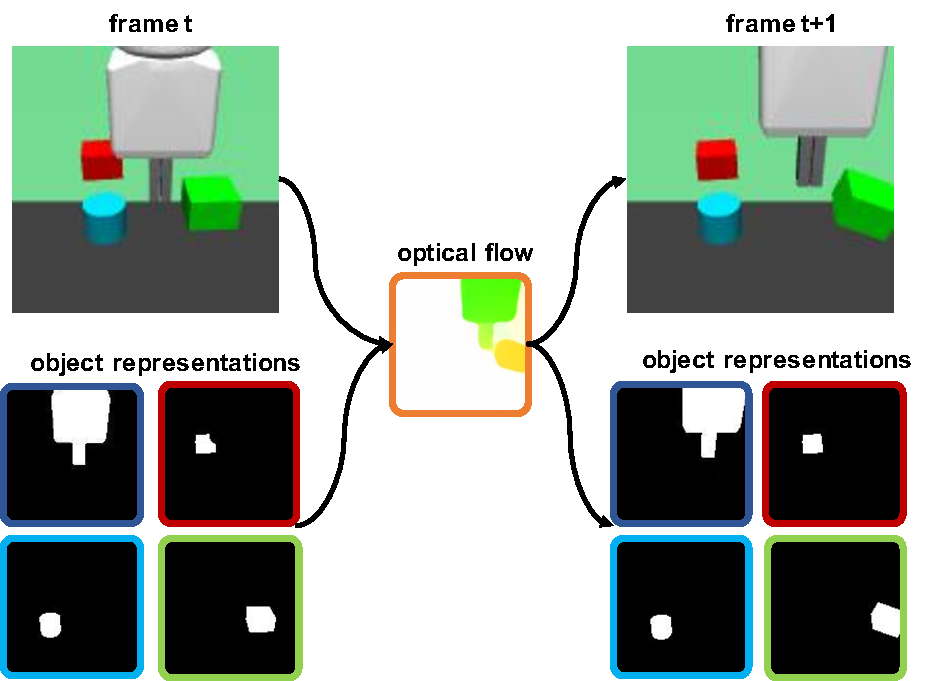
\includegraphics[width=8cm]{flood_main_figure.pdf}
    \caption{\jd{Introducing the idea that an optical flow warp applied to an object-structured representation should produce the object-structured representation of the next image}}
    \label{fig:desired_property}
\end{figure}

We evaluate \textsc{flood} on a variety of synthetic object discovery benchmarks used in previous works. In addition, we introduce a real-world tabletop robotic object pushing dataset. Our results show that \textsc{flood} yields reliable improvements over baseline methods based on reconstruction and contrastive losses, and even an approach that has access to additional information about the forces causing object motions in video.



%This does not rely on specific encoder architectures.

%, identifying correspondences between pixels in consecutive frames

%This naturally implements the principle of common fate: pixels that move together belong together.


% --- loosely, warping the discovered segmentation map of frame A with optical flow should 

%, identifying correspondences between pixels in consecutive frames

%first proposed by Gestalt psychologists (CITE): common fate --- ``pixels that move together belong together''. 

%In this context, we call back to an older family of work within cognitive science and computer vision. 

%on representations learned in unsupervised visual representation learning.  

%inas imposing structure on unsupervised representaions

%relevant information for most tasks, : how might computer vision systems learn to parse their world into objects


%Gestalt psychologists studying the cognitive bases of grouping studied 

%Gestalt common fate




\section{Flow-guided Object Discovery}
\label{sec:approach}

\begin{figure}
  \centering
  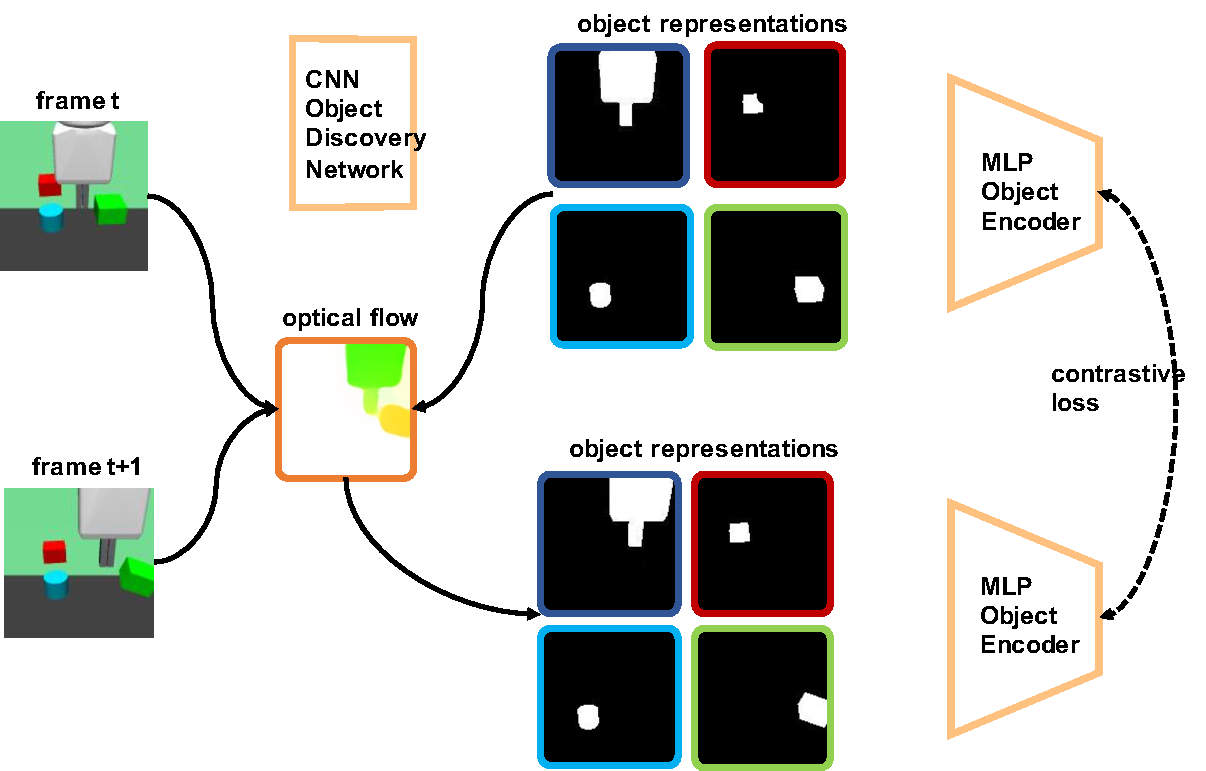
\includegraphics[width=8cm]{flood-network.pdf}

  \caption{Sample figure caption.}
  \label{fig:architecture}
\end{figure}

\jd{Suggestion for how to structure this: First, set up the problem and notation. What is given to you, and what is the goal? Then describe the slot encoder architecture and how objects are represented in slots. Should state that this is the representation used in C-SWM and resembles the representations used in other work. Our method is also compatible with other object representations, but we use this popular representation in our implementations. Next, we describe the desired property of those representations in terms of pixelwise flow i.e. warp ( mask ( frame 1)) = mask ( warp (frame 1)), where  warp(frame 1) = frame 2, and the warp is computed from optical flow. Next, we describe how this can be implemented using contrastive losses.}


Given some unlabeled video sequences, the goal of our method is to discover and learn object-centric representations with the help of motion information. Specifically, \textsc{flood} takes in an image input $f_t$, which is the video frame at time step $t$, and passing it through an object discovery network. This discovery network produces a set of feature maps $m_t = \{m_{t}^1, m_{t}^2, \dots. m_{t}^k \}$ around the discovered objects, where $k$ is the number of objects we expected. 

In order to take advantages of the motion information available in a video, \textsc{flood} takes in motion information provided by optical flow between two nearby frames $f_{t}$ and $f_{t'}$, and propagates the predicted feature maps $m_{t}$ to $\overline{m_{t'}}$. If the optical flow between these two frames are correct, we should expect that $\overline{m_{t'}}$ and $m_{t'}$ encodes the same object information. We could then use this property to train our object discovery network.

In this section, we first introduce our object discovery network. Next we describe our desired property of the learned representations in terms of optical flow. In the end we explain how to use these desired properties to train the object discovery network through contrastive learning. 

\subsection{Object Discovery Network}
The object discovery network $N_D$ takes in an image $f_t$, and outputs a set of $k$ feature maps $N_D(f_t) = m_t = \{m_{t}^1, m_{t}^2, \dots. m_{t}^k \}$. This networks is an CNN-based network, and the last activation layer is a sigmoid function. Thus each mask can be interpreted as a slot-wise segmentation mask that takes the value between 0-1. This slot-wise object representation is also used in ~\cite{kipf2019contrastive, locatello2020object}. Since it's a popular object representation in previous work, we adopt this in our implementation. \aq{I am afraid that if we say out method is also compatible with other object representations, reviewers are going to ask for results on other representations}

\subsection{Flow-guided Object Discovery Propagation}
As mentioned above, we believe that motion information in nearby video frames contain critical training signal for object discovery tasks. More specifically, given two nearby video frames $f_{t}$ and $f_{t'}$, the optical flow defines a map between frames: $h_{t \rightarrow t'}(f_t) = f_{t'}$ and $h_{t' \rightarrow t}(f_{t'}) = f_{t}$. This map defines a morphism and we can use it to propagate object information from one frame to another:
\[h_{t \rightarrow t'}(N_D(f_t)) = N_D(h_{t \rightarrow t'}(f_t))\],
where $h_{t \rightarrow t'}(N_D(f_t)) = \overline{m_{t'}}$ and $ N_D(h_{t \rightarrow t'}(f_t)) =  N_D(f_{t'}) = m_{t'}$.

If this morphism holds, then we know the following two conditions hold:  1) the map between frames($h_{t \rightarrow t'}$) is accurate, and 2) the object discovery feature maps are consistent across frames. The first condition is given by the precision of optical-flow prediction network. The second condition coincide with the training objective of our object discovery network. We next describe how to enforce this second condition via contrastive learning.

\subsection{Contrastive Learning}

\subsection{Implementation Detail}
A paragraph on implementation details somewhere. 

\section{Related Prior Work}
\label{sec:related_work}

%To move to after approach (?)

%Related work notes: 

\paragraph{Video object segmentation from motion and appearance.} As foreshadowed in Sec~\ref{sec:intro}, our approach for flow-guided object discovery is related to motion segmentation methods~\cite{shi1998motion,tron2007benchmark,yan2006general,tokmakov2017learning,keuper2018motion,bideau2018moa, yang2021rigidmask} in computer vision, which use optical flow cues to group pixels in video frames which move coherently together. Since purely flow-based groupings are not persistent and cannot handle static objects, video segmentation algorithms often combine these motion cues with appearance~\cite{weiss1995perceptually, jain2017fusionseg, tokmakov2017learning, cheng2017segflow}. However, all these methods are designed for segmenting video and can not handle static images as trained \textsc{flood} models do. Specifically, \textsc{flood} trains models appearance-based static image object segmentation models by using flow-based cues in training videos as a supervision signal.

% -- objects disappear once they stop moving. For more presistence, motion cues can be combined with appearance cues in video segmentation algorithms
%ALSO THE DEVA PAPER (?) 

\paragraph{Unsupervised representations from motion.} In the context of learning unsupervised representations, image region-level correspondences computed through object motion tracking~\cite{wang2015unsupervised} or by matching object-like regions~\cite{gao2016object} has been used before as a form of self-supervision. Compared to \textsc{flood}'s goal of discovering objects and forming object-structured representations of full images, they instead aim to train unstructured descriptors of objects and object-like regions in images. Most related to our approach from this literature, \citet{pathak2017learning} use motion segmentation of moving objects from video as targets for a single-image segmentation model. Note that this task is not well-posed; moving objects cannot be identified from a single image. Rather than produce a good segmentation model, this self-supervised segmentation task is merely intended as a ``pretext task''~\cite{pathak2017learning}, i.e., through training on this task, the CNN must acquire good unstructured image representations useful for other computer vision tasks.

%this is not a problem because they do not aim to train a segmentation model. Rather, 


\paragraph{Neural object discovery.} Nearly all neural object discovery approaches targeting general images or video are trained by reconstructing the input image~\cite{jakab2018unsupervised,jakab2020self,greff2019multi, burgess2019monet,locatello2020object,Kulkarni2019UnsupervisedLO, minderer2019unsupervised, engelcke2019genesis}, but two recent approaches are trained through contrastive losses to distinguish between distinct images in a dataset~\cite{racah2020slot,lowe2020learning}. \citet{racah2020slot} use temporal continuity in video for object discovery, in a method called slot-contrastive networks (SCN). Like \textsc{flood}, SCN uses temporally nearby frames as positives and distant frames as negatives, but it effectively treats nearby images as being identical since it does not account for pixel motions. Instead, as specified above, \textsc{flood} models nearby frames as related by a warp specified by optical flow. We compare against SCN in Sec~\ref{sec:experiments}.  %also uses a loss from the contrastive family, but guided by optical flow. 

In robotics contexts, where motion is attributable to known robot actions, several models~\cite{kipf2019contrastive, kipf2018neural, Veerapaneni2019EntityAI}, \jd{Aurora, could you look into the Veerapaneni paper?} use action-conditioned future prediction as a training objective for joint object discovery and environment dynamics modeling. The robot actions in these formulations help specify how the scenes in training videos evolve over time. \textsc{flood} replaces robot actions with dense pixel correspondences from optical flow, which are more general --- they specify how arbitrary videos evolve even with unknown actors and forces. Notably, our implementation of \textsc{flood} uses the popular object slot encoder architecture of contrastive structured world models (C-SWM)~\cite{kipf2019contrastive}, enabling a controlled comparison in Sec~\ref{sec:experiments}. With identical object encoders, and sans robot action knowledge, \textsc{flood} still performs comparably or better than C-SWM even in robotics datasets with known actions.

% We do not assume robot action knowledge so that \textsc{flood} remains more general and able to learn from uncontrolled video.

%. However, since they do not directly reason about motions, they simply approximate consecutive frames as being identical
%However, these are philosophically close antecedents of \textsc{flood}.

%Learning object descriptors in an unsupervised manner through tracking~\cite{wang2015unsupervised,gao2016object}


% %\subsection{Object Discovery}  
% \begin{itemize}[leftmargin=*]
%     %\item  \textsc{flood} falls into this latter category.
    
%     %\item None of these above approaches use motion as a signal for discovering objects. In the robotics contexts, some models aim to discover both objects and their dynamics under robot action assuming that robot actions are known. 
    
%     %\item 
    
%     %In particular, \citet{kipf2019contrastive} proposes a contrastive structured world model (C-SWM), several of whose architectural components we borrow.
    
%     \item 
    
%     % \item IODINE
%     % \item MONET
%     % \item GENESIS
%     % \item Slot Attention
% \end{itemize}
% and that they are the only cause of motion in the scene

% \subsection{Contrastive Learning}
% \begin{itemize}
%     \item InfoNCE
%     \item SimCLR
%     \item Moco
% \end{itemize}
% \subsection{Flow-based Representation Learning Method}
% \begin{itemize}
%     \item Unsupervised Learning of Visual Representations using Videos
% \end{itemize}
% \subsection{Motion Segmentation}


\section{Experiments}
\label{sec:experiments}

 

\subsection{Datasets}
\jd{If space, a figure up front just displaying a collection of images from each dataset to illustrate their corresponding visual domains.}

\subsection{Evaluation Metrics}
\textbf{Slot Accuracy}\\
\textbf{Slot Compactness}
\subsection{Training and Evaluation Settings}
\subsection{Baselines}

Throughout our approach we use three approaches as baselines, representing three different types of object discovery objectives from the literature. First, contrastive structured world models (\textbf{C-SWM})~\cite{kipf2019contrastive} represents joint object discovery and environment dynamics modeling through a future prediction approach. Slot attention (\textbf{SA})~\cite{locatello2020object} represents methods that learn representations using image reconstruction losses. Finally, slot-contrastive network (\textbf{SCN})~\cite{racah2020slot} uses temporal continuity as a signal for object discovery: it trains representations that can distinguish far-away frame pairs from nearby frame pairs, using a contrastive loss.  

All three baselines represent objects through a slot-based representation similar to \textsc{flood}, described in Sec~\ref{sec:approach}, making them well-suited for comparison. \textsc{flood} inherits the object encoder of C-SWM, which is also used in SCN. SA proposes a new attention-based architecture for encoding images into object slots.

%uses a new attention-based architecture to encode objects, and 

% \textbf{C-SWM}\\
% \textbf{Slot Contrastive Networks}\\
% \textbf{Slot Attention}

\subsection{Experiment Setup}

\subsection{Results}
\textbf{Question 1.} Does our method learn more accurate object centric representations?
Metrics: 1) Slot Accuracy 

\textbf{Question 2.} Does our method learn more disnentangled object-centric representations? Metrics: Slot compactness

\textbf{Question 3.} Robustness to the number of slots?

\jd{Prepare figures showing 1-2 nice examples for each dataset, perhaps a set of rows, where each row contains the input image, then the output masks of all baselines and our method for that image, similar to visualizations in papers like IODINE.}



\begin{table}
  \caption{Sample table title}
  \label{sample-table}
  \centering
  \begin{tabular}{lllll}
    \toprule
    \multicolumn{1}{c}{} & \multicolumn{4}{c}{3D Blocks} \\
    \cmidrule(r){2-5}  
      & MSE(Points)     & Slot Compactness     & Slot Modularity     & ARI  \\
    \midrule
    (Ours) &   &  &  &     \\
    C-SWM &    & &  &     \\
    Slot Contrastive &        & \\
    Slot Attention &    \\
    \bottomrule
  \end{tabular}
\end{table}
\begin{table}
  \caption{Sample table title}
  \label{sample-table}
  \centering
  \begin{tabular}{lllll}
    \toprule
    \multicolumn{1}{c}{} & \multicolumn{4}{c}{Simulated Control} \\
    \cmidrule(r){2-5}  
      & MSE(Points)$\downarrow$      & Slot Compactness$\uparrow$     & Slot Modularity$\uparrow$     & ARI$\uparrow$  \\
    \midrule
    (Ours) final s4 & 94.455135 &  0.38635144  & 0.0359788&0.41344     \\
    C-SWM not final &  &  0.45987  & 0.1717  &0.23062    \\
    Slot Contrastive final s4& 187.362204     & 0.098727525       & 0.05369954 & -\\
    Slot Attention &    \\
    \bottomrule
  \end{tabular}
\end{table}

\begin{table}
  \caption{Sample table title}
  \label{sample-table}
  \centering
  \begin{tabular}{lllll}
    \toprule
    \multicolumn{1}{c}{} & \multicolumn{4}{c}{Simulated Control} \\
    \cmidrule(r){2-5}  
      & \textsc{flood}(Ours)      & C-SWM    & Slot Contrastive     & Slot Attention  \\
    \midrule
   MSE(Points)$\downarrow$  & 100.86089 &  99.6055  & &      \\
   \midrule
    ARI$\uparrow$     &  0.5141849  & 0.398706  & - &   \\
    \bottomrule
  \end{tabular}
\end{table}

\begin{table}
  \caption{Sample table title}
  \label{sample-table}
  \centering
  \begin{tabular}{lllll}
    \toprule
    \multicolumn{1}{c}{} & \multicolumn{4}{c}{Real Control} \\
    \cmidrule(r){2-5}  
      & MSE(Points)$\downarrow$     & Slot Compactness$\uparrow$     & Slot Modularity$\uparrow$      & ARI$\uparrow$   \\
    \midrule
    (Ours) &  & & &    0.1685787 \\
    C-SWM &       &   &&  0.1596932    \\
    Slot Contrastive final s4 & 555.432067285/9.4475     &    0.11556364/0.1131474 &0.08461118/0.067329510 & - \\ 
    Slot Attention &  & &   \\
    \bottomrule
  \end{tabular}
\end{table}


\section{Conclusions}\label{sec:conclusions}


% \section{Citations, figures, tables, references}
% \label{others}

% These instructions apply to everyone.

% \subsection{Citations within the text}

% The \verb+natbib+ package will be loaded for you by default.  Citations may be
% author/year or numeric, as long as you maintain internal consistency.  As to the
% format of the references themselves, any style is acceptable as long as it is
% used consistently.

% The documentation for \verb+natbib+ may be found at
% \begin{center}
%   \url{http://mirrors.ctan.org/macros/latex/contrib/natbib/natnotes.pdf}
% \end{center}
% Of note is the command \verb+\citet+, which produces citations appropriate for
% use in inline text.  For example,
% \begin{verbatim}
%   \citet{hasselmo} investigated\dots
% \end{verbatim}
% produces
% \begin{quote}
%   Hasselmo, et al.\ (1995) investigated\dots
% \end{quote}

% If you wish to load the \verb+natbib+ package with options, you may add the
% following before loading the \verb+neurips_2021+ package:
% \begin{verbatim}
%   \PassOptionsToPackage{options}{natbib}
% \end{verbatim}

% If \verb+natbib+ clashes with another package you load, you can add the optional
% argument \verb+nonatbib+ when loading the style file:
% \begin{verbatim}
%   \usepackage[nonatbib]{neurips_2021}
% \end{verbatim}

% As submission is double blind, refer to your own published work in the third
% person. That is, use ``In the previous work of Jones et al.\ [4],'' not ``In our
% previous work [4].'' If you cite your other papers that are not widely available
% (e.g., a journal paper under review), use anonymous author names in the
% citation, e.g., an author of the form ``A.\ Anonymous.''

% \subsection{Footnotes}

% Footnotes should be used sparingly.  If you do require a footnote, indicate
% footnotes with a number\footnote{Sample of the first footnote.} in the
% text. Place the footnotes at the bottom of the page on which they appear.
% Precede the footnote with a horizontal rule of 2~inches (12~picas).

% Note that footnotes are properly typeset \emph{after} punctuation
% marks.\footnote{As in this example.}

% \subsection{Figures}

% \begin{figure}
%   \centering
%   \fbox{\rule[-.5cm]{0cm}{4cm} \rule[-.5cm]{4cm}{0cm}}
%   \caption{Sample figure caption.}
% \end{figure}

% All artwork must be neat, clean, and legible. Lines should be dark enough for
% purposes of reproduction. The figure number and caption always appear after the
% figure. Place one line space before the figure caption and one line space after
% the figure. The figure caption should be lower case (except for first word and
% proper nouns); figures are numbered consecutively.

% You may use color figures.  However, it is best for the figure captions and the
% paper body to be legible if the paper is printed in either black/white or in
% color.

% \subsection{Tables}

% All tables must be centered, neat, clean and legible.  The table number and
% title always appear before the table.  See Table~\ref{sample-table}.

% Place one line space before the table title, one line space after the
% table title, and one line space after the table. The table title must
% be lower case (except for first word and proper nouns); tables are
% numbered consecutively.

% Note that publication-quality tables \emph{do not contain vertical rules.} We
% strongly suggest the use of the \verb+booktabs+ package, which allows for
% typesetting high-quality, professional tables:
% \begin{center}
%   \url{https://www.ctan.org/pkg/booktabs}
% \end{center}
% This package was used to typeset Table~\ref{sample-table}.

% \begin{table}
%   \caption{Sample table title}
%   \label{sample-table}
%   \centering
%   \begin{tabular}{lll}
%     \toprule
%     \multicolumn{2}{c}{Part}                   \\
%     \cmidrule(r){1-2}
%     Name     & Description     & Size ($\mu$m) \\
%     \midrule
%     Dendrite & Input terminal  & $\sim$100     \\
%     Axon     & Output terminal & $\sim$10      \\
%     Soma     & Cell body       & up to $10^6$  \\
%     \bottomrule
%   \end{tabular}
% \end{table}

% \section{Final instructions}

% Do not change any aspects of the formatting parameters in the style files.  In
% particular, do not modify the width or length of the rectangle the text should
% fit into, and do not change font sizes (except perhaps in the
% \textbf{References} section; see below). Please note that pages should be
% numbered.

% \section{Preparing PDF files}

% Please prepare submission files with paper size ``US Letter,'' and not, for
% example, ``A4.''

% Fonts were the main cause of problems in the past years. Your PDF file must only
% contain Type 1 or Embedded TrueType fonts. Here are a few instructions to
% achieve this.

% \begin{itemize}

% \item You should directly generate PDF files using \verb+pdflatex+.

% \item You can check which fonts a PDF files uses.  In Acrobat Reader, select the
%   menu Files$>$Document Properties$>$Fonts and select Show All Fonts. You can
%   also use the program \verb+pdffonts+ which comes with \verb+xpdf+ and is
%   available out-of-the-box on most Linux machines.

% \item The IEEE has recommendations for generating PDF files whose fonts are also
%   acceptable for NeurIPS. Please see
%   \url{http://www.emfield.org/icuwb2010/downloads/IEEE-PDF-SpecV32.pdf}

% \item \verb+xfig+ "patterned" shapes are implemented with bitmap fonts.  Use
%   "solid" shapes instead.

% \item The \verb+\bbold+ package almost always uses bitmap fonts.  You should use
%   the equivalent AMS Fonts:
% \begin{verbatim}
%   \usepackage{amsfonts}
% \end{verbatim}
% followed by, e.g., \verb+\mathbb{R}+, \verb+\mathbb{N}+, or \verb+\mathbb{C}+
% for $\mathbb{R}$, $\mathbb{N}$ or $\mathbb{C}$.  You can also use the following
% workaround for reals, natural and complex:
% \begin{verbatim}
%   \newcommand{\RR}{I\!\!R} %real numbers
%   \newcommand{\Nat}{I\!\!N} %natural numbers
%   \newcommand{\CC}{I\!\!\!\!C} %complex numbers
% \end{verbatim}
% Note that \verb+amsfonts+ is automatically loaded by the \verb+amssymb+ package.

% \end{itemize}

% If your file contains type 3 fonts or non embedded TrueType fonts, we will ask
% you to fix it.

% \subsection{Margins in \LaTeX{}}

% Most of the margin problems come from figures positioned by hand using
% \verb+\special+ or other commands. We suggest using the command
% \verb+\includegraphics+ from the \verb+graphicx+ package. Always specify the
% figure width as a multiple of the line width as in the example below:
% \begin{verbatim}
%   \usepackage[pdftex]{graphicx} ...
%   \includegraphics[width=0.8\linewidth]{myfile.pdf}
% \end{verbatim}
% See Section 4.4 in the graphics bundle documentation
% (\url{http://mirrors.ctan.org/macros/latex/required/graphics/grfguide.pdf})

% A number of width problems arise when \LaTeX{} cannot properly hyphenate a
% line. Please give LaTeX hyphenation hints using the \verb+\-+ command when
% necessary.

% \begin{ack}
% Use unnumbered first level headings for the acknowledgments. All acknowledgments
% go at the end of the paper before the list of references. Moreover, you are required to declare
% funding (financial activities supporting the submitted work) and competing interests (related financial activities outside the submitted work).
% More information about this disclosure can be found at: \url{https://neurips.cc/Conferences/2021/PaperInformation/FundingDisclosure}.

% Do {\bf not} include this section in the anonymized submission, only in the final paper. You can use the \texttt{ack} environment provided in the style file to autmoatically hide this section in the anonymized submission.
% \end{ack}

% \section*{References}

% References follow the acknowledgments. Use unnumbered first-level heading for
% the references. Any choice of citation style is acceptable as long as you are
% consistent. It is permissible to reduce the font size to \verb+small+ (9 point)
% when listing the references.
% Note that the Reference section does not count towards the page limit.
% \medskip

\bibliography{refs}

%%%%%%%%%%%%%%%%%%%%%%%%%%%%%%%%%%%%%%%%%%%%%%%%%%%%%%%%%%%%
\section*{Checklist}

%%% BEGIN INSTRUCTIONS %%%
The checklist follows the references.  Please
read the checklist guidelines carefully for information on how to answer these
questions.  For each question, change the default \answerTODO{} to \answerYes{},
\answerNo{}, or \answerNA{}.  You are strongly encouraged to include a {\bf
justification to your answer}, either by referencing the appropriate section of
your paper or providing a brief inline description.  For example:
\begin{itemize}
  \item Did you include the license to the code and datasets? \answerYes{See Section~\ref{gen_inst}.}
  \item Did you include the license to the code and datasets? \answerNo{The code and the data are proprietary.}
  \item Did you include the license to the code and datasets? \answerNA{}
\end{itemize}
Please do not modify the questions and only use the provided macros for your
answers.  Note that the Checklist section does not count towards the page
limit.  In your paper, please delete this instructions block and only keep the
Checklist section heading above along with the questions/answers below.
%%% END INSTRUCTIONS %%%

\begin{enumerate}

\item For all authors...
\begin{enumerate}
  \item Do the main claims made in the abstract and introduction accurately reflect the paper's contributions and scope?
    \answerTODO{}
  \item Did you describe the limitations of your work?
    \answerTODO{}
  \item Did you discuss any potential negative societal impacts of your work?
    \answerTODO{}
  \item Have you read the ethics review guidelines and ensured that your paper conforms to them?
    \answerTODO{}
\end{enumerate}

\item If you are including theoretical results...
\begin{enumerate}
  \item Did you state the full set of assumptions of all theoretical results?
    \answerTODO{}
	\item Did you include complete proofs of all theoretical results?
    \answerTODO{}
\end{enumerate}

\item If you ran experiments...
\begin{enumerate}
  \item Did you include the code, data, and instructions needed to reproduce the main experimental results (either in the supplemental material or as a URL)?
    \answerTODO{}
  \item Did you specify all the training details (e.g., data splits, hyperparameters, how they were chosen)?
    \answerTODO{}
	\item Did you report error bars (e.g., with respect to the random seed after running experiments multiple times)?
    \answerTODO{}
	\item Did you include the total amount of compute and the type of resources used (e.g., type of GPUs, internal cluster, or cloud provider)?
    \answerTODO{}
\end{enumerate}

\item If you are using existing assets (e.g., code, data, models) or curating/releasing new assets...
\begin{enumerate}
  \item If your work uses existing assets, did you cite the creators?
    \answerTODO{}
  \item Did you mention the license of the assets?
    \answerTODO{}
  \item Did you include any new assets either in the supplemental material or as a URL?
    \answerTODO{}
  \item Did you discuss whether and how consent was obtained from people whose data you're using/curating?
    \answerTODO{}
  \item Did you discuss whether the data you are using/curating contains personally identifiable information or offensive content?
    \answerTODO{}
\end{enumerate}

\item If you used crowdsourcing or conducted research with human subjects...
\begin{enumerate}
  \item Did you include the full text of instructions given to participants and screenshots, if applicable?
    \answerTODO{}
  \item Did you describe any potential participant risks, with links to Institutional Review Board (IRB) approvals, if applicable?
    \answerTODO{}
  \item Did you include the estimated hourly wage paid to participants and the total amount spent on participant compensation?
    \answerTODO{}
\end{enumerate}

\end{enumerate}

%%%%%%%%%%%%%%%%%%%%%%%%%%%%%%%%%%%%%%%%%%%%%%%%%%%%%%%%%%%%

\appendix

\section{Appendix}

Optionally include extra information (complete proofs, additional experiments and plots) in the appendix.
This section will often be part of the supplemental material.

\end{document}